\section{Transistores}

faltan los tipos y eso... lo vimos en una clase, aunque dijo el profesor que no ibamos a verlos, solo los mencionaba, de todas maneras, no estaría demás mencionarlo nosotros también... o qué consideran?
\subsection{Transistores bipolares}

introducción?
\subsubsection{Construcción}


En la construcción de los transistores hoy en día se emplean materiales como germanio (Ge), silicio (Si), arseniuro de galio (GaAs) o aleaciones de silicio y germanio o silicio y aluminio.

El material es dopado con otras sustancias que le permitan tener un exceso de electrones o un déficit de los mismos (vacantes
), para así formar capas en forma de ``sandwich''.\\



Por ejemplo, para el caso del Silicio mostrado en la figura \ref{fig:silicio} si es dopado con Fósforo (P) (extremo derecho de la \ref{fig:silicio-dopado}), por cada átomo de fósforo existirá un electrón excedente; si es dopado con Aluminio (Al), existirá una vacante (extremo izquierdo de la \ref{fig:silicio-dopado}).


Este juego entre electrones excedentes y vacantes representa el funcionamiento principal de los transistores bipolares.


\begin{figure}[H]
	\centering
	\begin{subfigure}[b]{.45\linewidth}
		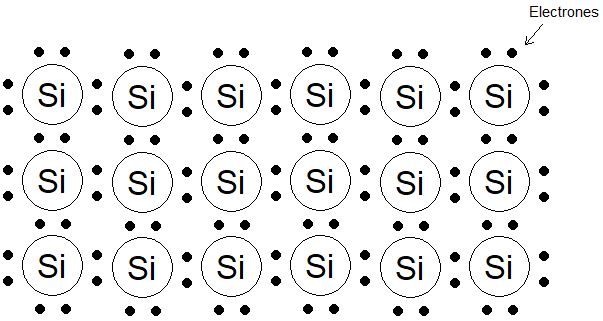
\includegraphics[width=\linewidth]{silicio}
		\caption{Silicio sin dopar}
		\label{fig:silicio}
	\end{subfigure}
	\begin{subfigure}[b]{.45\linewidth}
		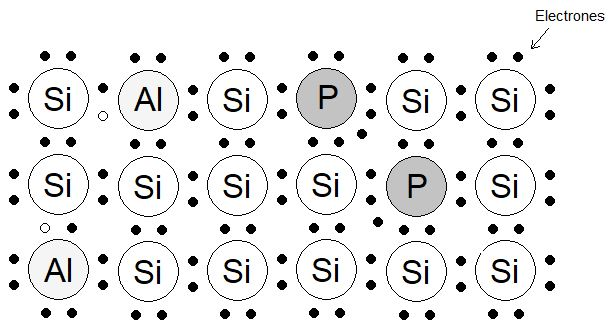
\includegraphics[width=\linewidth]{silicio-dopaje}
		\caption{Silicio dopado}
		\label{fig:silicio-dopado}
	\end{subfigure}
\end{figure}



Cuando el material tiene un excedente de electrones se dice que es \textsl{tipo n}, y cuando tiene vacantes es de \textsl{tipo p}. Con esto en mente, existen dos configuraciones en la construcción de un transistor:

\begin{itemize}
	\item \textbf{pnp:} dos capas externas de material tipo p y una capa delgada interna de material tipo n;
	\item \textbf{npn:} dos capas externas de material tipo n y una capa delgada interna de material tipo p.
\end{itemize}

\begin{figure}[H]
	\centering
	\begin{subfigure}[b]{.4\linewidth}
		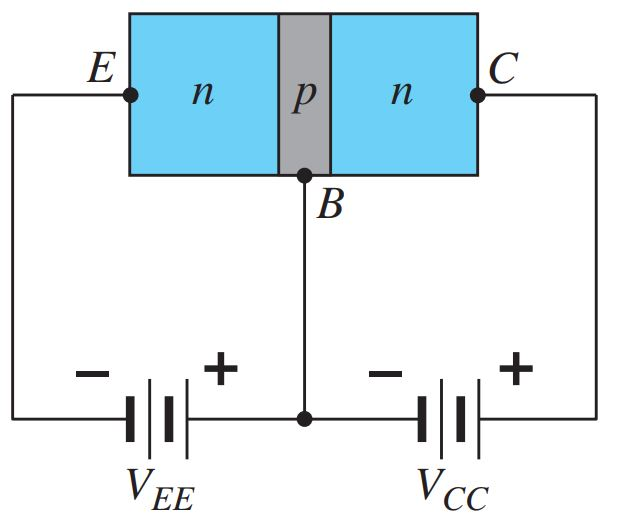
\includegraphics[width= .9\linewidth]{npn}
		\caption{Tipo NPN}
	\end{subfigure}
	\begin{subfigure}[b]{.4\linewidth}
		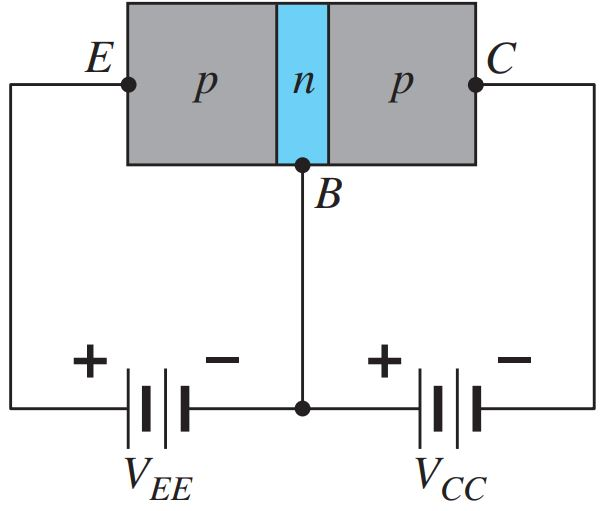
\includegraphics[width= .9\linewidth]{pnp}
		\caption{Tipo PNP}
	\end{subfigure}
	\caption{Transistores bipolares}
	\label{fig:transistores}
\end{figure}

Con la polarización mostrada en la figura \ref{fig:transistores}, las terminales se identificaron por medio de las
letras mayúsculas E para \textsl{emisor}, C para \textsl{colector} y B para \textsl{base}.\\

La capa del emisor está muy dopada, la base ligeramente, y el colector está moderadamente dopado, más que la base y menos que el emisor. \\
(Propósito de por qué ese dopaje)

\subsubsection{Union pn}

En los transistores hay dos uniones pn.\\

Tension que se forma en la unión.
Para el silicio, 0,7V...\\

Falta completar

\subsubsection{Ganancia de corriente $\beta$}

\begin{equation}
	\beta = \dfrac{i_C}{i_B}
\end{equation}